%!TeX root = main.tex
%!encoding = UTF-8 Unicode

\subsection{Probe Architecture and Implementation}

To meet the combined requirements for low insertion resistance, high-frequency response, and a defined output level (Section~\ref{sec:CurrentRequirements}), an active shunt design was chosen.
The active-shunt concept is adapted from~\cite{shillaber_gigahertz_2020,shillaber_ultrafast_2022}; its dual-channel arrangement follows the voltage-probe architecture in Section~\ref{sec:design_voltage}.
\fref{fig:ESBActiveShunt} shows the three stages of the probe:
\begin{enumerate}
	\item Passive shunt element for low-intrusion current sensing
	\item Active compensation and amplification of the shunt signal
	\item Dual-channel subtractor stage:
	\begin{enumerate}
		\item Low-pass signal path for conventional switching analysis
		\item High-pass signal path for high-frequency emission analysis
	\end{enumerate}
\end{enumerate}


\begin{figure}[htbp]
	\centering
	\tikzsetnextfilename{Diss_CompensatedCurrentShunt}
	\import{./figures/5_CurrentProbe/}{"Diss_CompensatedCurrentShunt.pdf_tex"}
	\caption{Simplified schematic overview of active current shunt.}\label{fig:ESBActiveShunt}
\end{figure}

The active shunt is integrated into the power board, which also carries the half-bridge.
The PCB photograph in \fref{fig:ESBActiveShuntPhoto} shows the physical arrangement of the signal chain: the passive shunt sits beside the low-side DUT \mi{Q}{LS}, followed by the compensation circuit and the separate low-pass and high-pass paths.
The DAVP connector, gate driver, and active shunt power supply are also shown.
The three probe stages are described in detail below.


\begin{figure}[ht]
	\centering
	\import{./figures/5_CurrentProbe/}{"Diss_Pic_AShunt.pdf_tex"}
	\caption{PCB implementation of the active current shunt and associated circuitry.}\label{fig:ESBActiveShuntPhoto}
\end{figure}

\subsubsection*{Passive Shunt Element}

The passive sensing element must measure current without substantially damping the commutation loop.
This requires a low shunt resistance, but the element's parasitic inductance limits the bandwidth over which its voltage remains proportional to current.
For a shunt resistance \mi{R}{shunt} and parasitic inductance \mi{L}{shunt}, this bandwidth is
\begin{equation}
	\mi{f}{bw,shunt} = \frac{1}{2\pi \tau_\text{shunt}} = \frac{\mi{R}{shunt}}{2\pi\mi{L}{shunt}}
	\label{eq:fbw_shunt}
\end{equation}
The relation therefore creates a trade-off between low insertion resistance and passive sensing bandwidth.

Increasing the shunt resistance raises its passive bandwidth but also increases damping in the commutation loop.
Conventional passive shunts targeting high bandwidth consequently use comparatively high resistances, which are unsuitable for low-intrusion EMC analysis.
For a parasitic inductance of \SI{250}{pH}, representative of a 0612 shunt package, \fref{fig:Diss_Current_PassiveShuntCalc} illustrates the trade-off.
At \SI{1}{m\ohm}, the bandwidth is approximately \SI{636}{kHz}; reaching \SI{500}{MHz} would require approximately \SI{0.79}{\ohm}.
Increasing resistance alone therefore cannot meet the bandwidth target without sacrificing low insertion resistance.

\begin{figure}[ht]
	\centering
	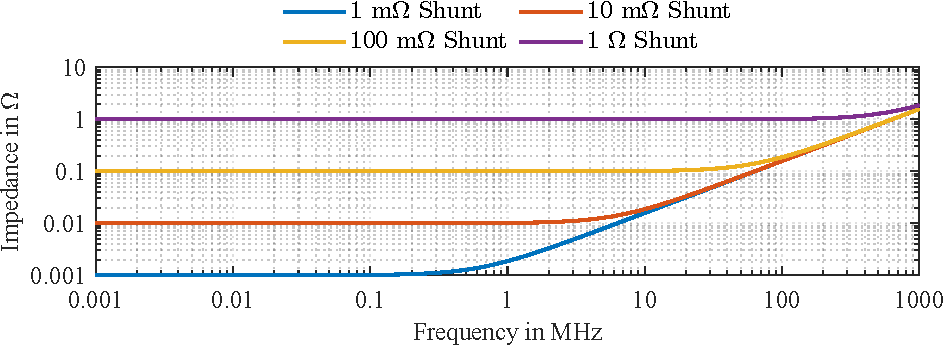
\includegraphics[scale=1]{figures/5_CurrentProbe/Diss_Current_PassiveShuntCalc.pdf}
	\caption{Achievable bandwidth of a passive current shunt with a parasitic inductance of \SI{250}{pH} as a function of the shunt resistance.}\label{fig:Diss_Current_PassiveShuntCalc}
\end{figure}

Reducing parasitic inductance alone does not remove this trade-off.
Physical dimensions and current-carrying capability constrain the achievable inductance.
Even the \SI{150}{pH} reported for a coaxial shunt~\cite{wang_high_} gives only approximately \SI{2}{MHz} at \SI{2}{m\ohm}.
The sensing element is therefore designed for low insertion resistance, while the subsequent active stage compensates for its inductive frequency response.

Ten parallel-connected metal-foil resistors provide the low insertion resistance of the passive sensing element.
Each resistor has a resistance of \SI{20}{m\ohm} in a 0508 package, giving a total sense resistance of \SI{2}{m\ohm}.
The resulting resistance satisfies the insertion-resistance limit in Section~\ref{sec:CurrentRequirements}.
\fref{fig:ESBPassiveShunt} shows the layout and implemented PCB, while \tref{tab:ShuntParameters} summarizes the shunt parameters.

\begin{figure}[ht]
	\centering
	\tikzsetnextfilename{Diss_PassiveShuntPCB_3D_wSchematic}
	\import{./figures/5_CurrentProbe/}{"Diss_PassiveShuntPCB_3D_wSchematic.pdf_tex"}
	\caption{Design of passive part of the current shunt.}\label{fig:ESBPassiveShunt}
\end{figure}

\begin{table}[ht]
	\caption{Parameter values of the passive shunt element}
	\label{tab:ShuntParameters}
	\centering
	\begin{tabular}{ll}
		\toprule
		\textbf{Parameter} &  \textbf{Value} \\
		\midrule
		\mi{R}{shunt} & \SI{2}{m\Omega} \\
		\mi{L}{shunt,calc} & \SI{24}{pH} \\
		\mti{G}{shunt} & \SI{2}{mV/A} \\
		\bottomrule
	\end{tabular}
\end{table}

The resistor arrangement reduces parasitic inductance by keeping the forward and return current paths close together.
Current flows along the bottom of the chosen metal-foil resistor packages, allowing a nearby return path in the PCB.
A semicircular arrangement places the vias along the outer edge of the resistor group.
Return current flows directly beneath the resistors and then vertically toward the DC-link capacitors.
Following the approach in~\cite{shillaber_gigahertz_2020}, this geometry reduces loop area and increases mutual coupling between the forward and return paths.

Unlike shunt designs that impose a limit on the inductance added to the commutation loop, this design does not require a specific value for that contribution.
The DUT is characterized for the assembled board's effective commutation-loop inductance \mi{L}{\sigma}, including the shunt's contribution.
The shunt's parasitic inductance still affects its transfer function and must be accounted for in the compensation circuit.
A surface-mount MMCX connector enables measurement of the passive shunt's transfer function.
The measured response is used to select the component values of the subsequent compensation stage.

Coupling into the shunt-to-amplifier connection was observed in an earlier design.
To limit this error source, buried traces in the two middle layers of the 4-layer PCB carry the small shunt signal.
A surrounding via fence connects the top and bottom ground planes along this path.
The signal is referenced to the negative DC-link potential rather than the DUT's Kelvin-source terminal.
Together, the buried traces and via fence shield the signal before it reaches the compensation amplifier.



\FloatBarrier

\subsubsection*{Active Compensation Amplifier}
The compensation amplifier counteracts the shunt's inductive frequency response.
Above the shunt's characteristic frequency, its parasitic inductance causes the sensed voltage to rise relative to the resistive response.
A differential low-pass network offsets this rise so that the output remains proportional to current over the usable frequency range.
The circuit is shown in \fref{fig:ESBCompensation}, with component values listed in \tref{tab:CompensationParameters}.

\begin{figure}[ht]
	\centering
	\tikzsetnextfilename{Diss_Compensation_Shunt_ESB}
	\import{./figures/5_CurrentProbe/}{"Diss_Compensation_Shunt_ESB.pdf_tex"}
	\caption{Circuit of the active current-shunt compensation stage.}\label{fig:ESBCompensation}
\end{figure}


\begin{table}[ht]
	\caption{Component values of the active compensation stage}
	\label{tab:CompensationParameters}
	\centering
	\begin{tabular}{ll}
		\toprule
		\textbf{Parameter} &  \textbf{Value} \\
		\midrule
		\mi{L}{comp,p}, \mi{L}{comp,n} & \SI{82}{nH} \\
		\mi{R}{comp,p}, \mi{R}{comp,n} & \SI{13}{\Omega} \\
		\bottomrule
	\end{tabular}
	\hspace{1cm}
	\begin{tabular}{ll}
		\toprule
		\textbf{Parameter} &  \textbf{Value} \\
		\midrule
		\mti{OP}{comp} & LTC6409 \\
		\mi{R}{1}, \mi{R}{2} & \SI{75}{\Omega} \\
		\mi{R}{3}, \mi{R}{4} & \SI{120}{\Omega} \\
		\mi{C}{1}, \mi{C}{2} & \SI{1.3}{pF} \\
		\mi{R}{5}, \mi{R}{6} & \SI{10}{\ohm} \\
		\mti{G}{comp}  & 1.6 \\
		\bottomrule
	\end{tabular}
\end{table}


In the idealized model, a flat response requires the compensation network's pole to coincide with the shunt's zero.
This condition matches the characteristic frequencies of the two networks.
The series inductance \mi{L}{comp} and resistance \mi{R}{comp} set the compensation frequency.
The matching condition is
\begin{align}
	\mi{f}{shunt} &\stackrel{!}{=} \mi{f}{comp} \\
	\frac{\mi{R}{shunt}}{2\pi \mi{L}{shunt}} &= \frac{\mi{R}{comp,eff}}{2\pi \mi{L}{comp}} \label{eq:compensation}
\end{align}

The effective resistance \mi{R}{comp,eff} accounts for loading by the amplifier's resistor network:
\begin{align}
	\mi{R}{comp,eff} &= \mi{R}{comp} || (\mi{R}{1}+\mi{R}{3}) \\
					 &\approx \mi{R}{comp} \hspace{2.5cm}, \text{for } \mi{R}{comp} \ll (\mi{R}{1}+\mi{R}{3})
\end{align}

When \mi{R}{comp} is small compared with the loading resistance, the matching condition gives the approximate compensation inductance:
\begin{equation}
	\mi{L}{comp} \approx \mi{L}{shunt}\cdot\frac{\mi{R}{comp}}{\mi{R}{shunt}}.
\end{equation}

VNA measurements guide the adjustment of the compensation network.
Transmission is measured from the MMCX input \mi{v}{shunt} to the compensation-stage output \mi{v}{comp}.
For single-ended acquisition, \mi{v}{comp+} connects to the VNA input.
The other output, \mi{v}{comp-}, is terminated to ground through \SI{50}{\ohm}, so both amplifier outputs see the same load.
\fref{fig:VNA_AShunt_comp} compares the responses with and without the discrete compensation inductor.

The response without the discrete inductor does not isolate the shunt's parasitic inductance.
Its characteristic frequency is approximately \SI{10}{MHz}, corresponding to an apparent shunt inductance of \SI{32}{pH}.
However, the shunt-to-amplifier traces contribute inductance and already provide partial compensation.
The apparent \SI{32}{pH} therefore cannot be attributed to the passive shunt alone.

\begin{figure}[ht]
	\centering
	\input{"figures/5_CurrentProbe/VNA_AShunt_comp.tex"}
	\caption{Frequency response with and without the discrete compensation inductor, illustrating compensation of the passive shunt's inductive response.}\label{fig:VNA_AShunt_comp}
\end{figure}

The measured response is compensated with a discrete inductance of \SI{82}{nH} and a compensation resistance of \SI{13}{\ohm}.
Buried differential traces of \SI{2.5}{cm} contribute a calculated additional inductance of approximately \SI{75}{nH}~\cite{vielspassspaeter}.
Including the trace inductance in the effective compensation inductance gives the following shunt-inductance estimate from \eref{eq:compensation}:

\begin{equation}
	\mi{L}{shunt,calc} = \frac{\mi{R}{shunt}}{\mi{R}{comp}}\cdot \mi{L}{comp,eff} = \frac{\SI{2}{m\Omega}}{\SI{13}{\Omega}}\cdot (\SI{82}{nH}+\SI{75}{nH}) = \SI{24}{pH}
\end{equation}

The amplifier's gain and phase correction are chosen to preserve its usable frequency response.
Moderate gain limits the bandwidth penalty of amplification.
The resistor ratio sets its gain:
\begin{equation}
	\mti{G}{comp} = \frac{\mi{R}{3}}{\mi{R}{1}} = 1.6.
\end{equation}
Capacitors \mi{C}{1} and \mi{C}{2} compensate for the phase shift associated with parasitic input capacitance.
Both capacitors are trimmed to \SI{1.3}{pF} for this layout.

The compensated response does not remain flat across the full \SI{500}{MHz} target range.
In \fref{fig:VNA_AShunt_comp}, the measured response stays only up to \SI{369}{MHz} within the \SI{3}{dB} band.
Measurements of all four $S$-parameters in \fref{fig:VNA_AShunt_comp_S} help identify the root cause.
Reverse transmission \mti{S}{12} increases above approximately \SI{300}{MHz}, indicating a parsitic, parallel, passive path between the amplifier input and output.
This additional signal path can alter the intended response at high frequencies.

\begin{figure}[ht]
	\centering
	\input{"figures/5_CurrentProbe/VNA_AShunt_comp_S.tex"}
	\caption{Measured $S$-parameters from the shunt measurement port to the compensation-amplifier output.}\label{fig:VNA_AShunt_comp_S}
\end{figure}

Reducing the relative influence of the passive path requires a trade-off between insertion resistance, amplifier gain and amplifier bandwidth.
Increasing \mi{R}{shunt} would raise the sensed voltage but violate the insertion-resistance limit.
Increasing compensation-stage gain would reduce usable bandwidth because of the amplifier's finite gain-bandwidth product.
Additional gain is therefore assigned to the subsequent filter stages rather than concentrated in the compensation amplifier.
The effect of downstream gain on the low-pass response is examined in Section~\ref{sec:CurrentVerification}.


\FloatBarrier

\subsubsection*{Dual-Channel Filter Stage}
The dual-channel stage conditions the compensated current signal for switching and high-frequency emission analysis.
Following the voltage-probe architecture in Section~\ref{sec:design_voltage}, the signal enters separate low-pass and high-pass paths.
The low-pass path preserves the switching waveform for conventional switching metrics.
The high-pass path suppresses dominant low-frequency content to improve resolution of small high-frequency current components.
Each path provides an output for oscilloscope acquisition.

\subsubsection*{Low-Pass Path}
The low-pass path amplifies the compensated current signal for time-domain switching analysis.
A fully-differential amplifier subtracts the two compensation-stage outputs and amplifies their difference.
\fref{fig:ESBLowpass} shows the circuit, and \tref{tab:LowPassParameters_Shunt} lists its component values.

\begin{figure}[ht]
	\centering
	\tikzsetnextfilename{Diss_Lowpass_Shunt_ESB}
	\import{./figures/5_CurrentProbe/}{"Diss_Lowpass_Shunt_ESB.pdf_tex"}
	\caption{Circuit of the active current-shunt low-pass stage.}\label{fig:ESBLowpass}
\end{figure}
\FloatBarrier

Single-ended acquisition of the oscilloscope input uses one of the low-pass amplifier's two differential outputs.
The oscilloscope loads this output with \SI{50}{\ohm}.
The other output is terminated to ground through \mi{R}{12} = \SI{60}{\ohm}, matching the series combination of \mi{R}{11} and the oscilloscope input.
This balance helps preserve common-mode rejection.

The following nominal gain and transimpedance expressions assume symmetric resistor values in both differential branches.
Here, \mi{R}{5} = \mi{R}{6}, \mi{R}{7} = \mi{R}{8}, and \mi{R}{9} = \mi{R}{10}, as implemented in this design.
Because only one output is measured, its voltage is half the differential output voltage.
The resulting low-pass stage gain is
\begin{equation}
	\mti{G}{LP} = \frac{\mi{v}{LP}}{\mi{v}{comp}} = \frac{1}{2}\cdot\frac{\mi{R}{9}}{\mi{R}{7}+\mi{R}{5}} = 2.25,
\end{equation}
The compensation amplifier's output resistor \mi{R}{5} is in series with the subtractor input resistor \mi{R}{7}, giving an effective input resistance of \mi{R}{7}+\mi{R}{5}.

The output resistor \mi{R}{11} forms a voltage divider with the oscilloscope input resistance \mi{R}{osci}.
The fraction of the amplifier output measured at the oscilloscope is
\begin{equation}
	\mti{G}{out} = \frac{\mi{R}{osci}}{\mi{R}{11} + \mi{R}{osci}} = \frac{\SI{50}{\Omega}}{\SI{10}{\Omega} + \SI{50}{\Omega}} = 0.83,
\end{equation}

Combining the shunt sensitivity, amplifier gains, and output divider gives the nominal low-frequency transimpedance at the oscilloscope:
\begin{align}
	\frac{\mi{v}{LP}}{\mi{i}{S}} &= \mti{G}{shunt}\cdot\mti{G}{comp}\cdot\mti{G}{LP}\cdot\mti{G}{out} \\
				&= \SI{2}{mV/A}\cdot 1.6\cdot 2.25\cdot 0.83 \\
				&= \SI{6}{mV/A}.
\end{align}

The nominal transimpedance determines the output voltage for a given shunt current.
To acquire the amplified switching waveform without clipping, the low-pass amplifier needs sufficient output swing.
It therefore uses a higher supply range (\SI{\pm5}{\volt}) than the compensation and high-pass amplifiers.
The larger output signal also provides more margin above the oscilloscope noise floor.
The amplifier choice comes at the cost of bandwidth, but low-pass analysis is limited to spectral components distinguishable above the noise floor.

\begin{table}[ht]
	\caption{Component values of the low-pass amplifier stage}
	\label{tab:LowPassParameters_Shunt}
	\centering
	\begin{tabular}{ll}
		\toprule
		\textbf{Parameter} &  \textbf{Value} \\
		\midrule
		\mti{OP}{LP} & OPA817 \\
		\mi{R}{7}, \mi{R}{8} & \SI{30}{\Omega} \\
		\mi{R}{9}, \mi{R}{10} & \SI{180}{\Omega} \\
		\mi{R}{11} & \SI{10}{\Omega} \\
		\mi{R}{12} & \SI{60}{\Omega} \\
		\bottomrule
	\end{tabular}
\end{table}
\FloatBarrier

\subsubsection*{High-Pass Path}
The high-pass path equalizes the commutation-current spectrum to resolve small high-frequency components.
The current spectrum falls by approximately \SI{-40}{dB/dec}.
Two cascaded first-order high-pass stages provide an approximately \SI{+40}{dB/dec} rising response below their corner frequencies.
This equalization reduces the amplitude range presented to the oscilloscope.
As in the voltage probe, the path is not intended to reproduce the original time-domain waveform.
The circuit and component values are shown in \fref{fig:ESBHighpass} and \tref{tab:ComponentsHighPass_Shunt}.

\begin{figure}[ht]
	\centering
	\tikzsetnextfilename{Diss_Highpass_Shunt_ESB}
	\import{./figures/5_CurrentProbe/}{"Diss_Highpass_Shunt_ESB.pdf_tex"}
	\caption{Circuit of the active current-shunt high-pass path.}\label{fig:ESBHighpass}
\end{figure}


The two LTC6409 stages form the second-order high-pass response.
The first stage, \mti{OP}{HP1}, provides the first high-pass response.
The second stage, \mti{OP}{HP2}, adds the second high-pass response.
Their equal nominal $RC$ values place both corner frequencies at the same frequency.

The high-pass corner frequencies lie above the intended measurement range so that acquisition occurs on the rising response.
Including the compensation-stage output resistor \mi{R}{5}, the first-stage input pole is
\begin{equation}
	\mi{f}{HP,1} = \frac{1}{2\pi (\mi{R}{5}+\mi{R}{13})\mi{C}{7}} \approx \SI{663}{MHz}.
\end{equation}
The second stage has the same nominal input pole because \mi{R}{17} = \mi{R}{5}, \mi{R}{19} = \mi{R}{13}, and \mi{C}{11} = \mi{C}{7}.
Well below these input poles, the two stages together approach the intended \SI{+40}{dB/dec} slope.
% Near the corners, the response deviates from this slope and must be determined by calibration.

The final stage, \mti{OP}{HP3}, converts the differential signal to a single-ended output for \SI{50}{\ohm} acquisition.
Matched resistor ratios in its positive and negative input branches give both signals equal gain.
This balance is necessary for the output to represent their amplified difference.

For ideal amplifiers, the stage transfer functions include the series output resistors of the preceding stages.
Capacitors \mi{C}{9}, \mi{C}{10}, \mi{C}{13}, and \mi{C}{14} trim the amplifier poles and are omitted from this nominal model:
\begin{align}
	\mti{G}{HP1}(s) &= \frac{s\mi{C}{7}\mi{R}{15}}{1+s\mi{C}{7}(\mi{R}{5}+\mi{R}{13})} \\
	\mti{G}{HP2}(s) &= \frac{s\mi{C}{11}\mi{R}{21}}{1+s\mi{C}{11}(\mi{R}{17}+\mi{R}{19})} \\
	\mti{G}{HP3} &= \frac{\mi{R}{f}}{\mi{R}{24}+\mi{R}{g}} \\
	\mti{G}{out} &= \frac{\mi{R}{osci}}{\mi{R}{27}+\mi{R}{osci}}.
\end{align}
Here, \mi{R}{osci} is the \SI{50}{\ohm} oscilloscope input resistance.
The current high-pass path prioritizes gain because the low-resistance shunt produces a much smaller signal than the voltage probe.
In the voltage probe, the stage gains can be distributed to improve noise performance.
Here, the small current-probe signal requires as much amplification as the usable bandwidth permits.
Both high-pass stages therefore use equal resistor-only gain ratios of 6.5.
Increasing either gain further would reduce usable bandwidth because of the finite gain-bandwidth product.
The selected distribution thus prioritizes the oscilloscope signal level under the bandwidth constraint.

The gain at the oscilloscope is the product of the three stage gains and the output-loading factor:
\begin{equation}
	\mti{G}{HP,osci}(s) = \frac{\mi{v}{HP,osci}(s)}{\mi{v}{comp}(s)} = \mti{G}{HP1}(s)\cdot\mti{G}{HP2}(s)\cdot\mti{G}{HP3}\cdot\mti{G}{out}.
\end{equation}

Above the input poles, the nominal transfer functions approach resistor-limited gains.
Finite amplifier bandwidth can limit the realized response before those poles are reached.
The usable equalization range must therefore be established by the small-signal verification in Section~\ref{sec:CurrentVerification}.



\begin{table}[ht]
	\caption{Component values of the high-pass path}
	\label{tab:ComponentsHighPass_Shunt}
	\centering
	\begin{tabular}[t]{l l}
		\toprule
		\textbf{Parameter} & \textbf{Value}\\
		\midrule
		\mti{OP}{HP1} & LTC6409\\
		\mi{C}{7}, \mi{C}{8} & \SI{6}{pF}\\
		\mi{R}{13}, \mi{R}{14} & \SI{30}{\Omega}\\
		\mi{R}{15}, \mi{R}{16} & \SI{260}{\Omega}\\	
		\mi{C}{9}, \mi{C}{10} & \SI{0.8}{pF}\\
		\mi{R}{17}, \mi{R}{18} & \SI{10}{\Omega}\\
		\bottomrule
	\end{tabular}
	\hspace{0.5cm}
	\begin{tabular}[t]{l l} 
		\toprule
		\textbf{Parameter} & \textbf{Value}\\
		\midrule
		\mti{OP}{HP2} & LTC6409\\
		\mi{C}{11}, \mi{C}{12} & \SI{6}{pF}\\
		\mi{R}{19}, \mi{R}{20} & \SI{30}{\Omega}\\		
		\mi{R}{21}, \mi{R}{22} & \SI{260}{\Omega}\\		
		\mi{C}{13}, \mi{C}{14} & \SI{0.8}{pF}\\
		\mi{R}{23}, \mi{R}{24} & \SI{10}{\Omega}\\
		\bottomrule
	\end{tabular}
	\hspace{0.5cm}
	\begin{tabular}[t]{l l}
		\toprule
		\textbf{Parameter} & \textbf{Value}\\
		\midrule
		\mti{OP}{HP3} & THS4302\\
		\mi{R}{25} & \SI{50}{\Omega}\\		
		\mi{R}{26} & \SI{200}{\Omega}\\
		\mi{R}{g} & \SI{50}{\Omega}\\		
		\mi{R}{f} & \SI{200}{\Omega}\\	
		\mi{R}{27} & \SI{10}{\Omega}\\
		\bottomrule
	\end{tabular}
\end{table}



\FloatBarrier

\subsubsection*{Shielding Concept and Implementation}
The active shunt requires shielding along its sense connection and around its amplifier circuitry because both are close to the switching node.
The shunt-to-amplifier connection is particularly sensitive because it carries a small voltage.
Buried differential traces carry \mi{v}{shunt} between the PCB ground planes.
A surrounding via fence connects the planes, forming a coaxial-style connection.
This routing helps limit pickup before the signal reaches the compensation amplifier.

A custom-made nickel-silver-alloy EMC shield limits coupling from the switching node into the active circuitry.
Its PCB mounting connections reference the shield to analog ground.
These connections are visible in \fref{fig:ESBActiveShuntPhoto}, which shows the board before the shield is installed.
The buried routing and grounded shield thus address coupling along the sense connection and into the active circuitry, respectively.
Switching tests in Section~\ref{sec:CurrentVerification} assess the external shield's influence on the measured waveform.